\section{Proposed Framework} \label{sec:Technical}
The main objective of this work is to create a generic framework for Supply Chain Management (SCM). Árion project is divided into three main modules described below: Frond-End WebApp, Back-End WebApp, and Data Storage. Figure~\ref{fig:detalhamentotecnico} shows the application architecture and its components. An SCM platform relies on three main items: assets, steps, and actors. Our approach is based on this triad, that must be defined on the creation of a new supply chain.

%htbp
\begin{figure}[ht]
\begin{center}
  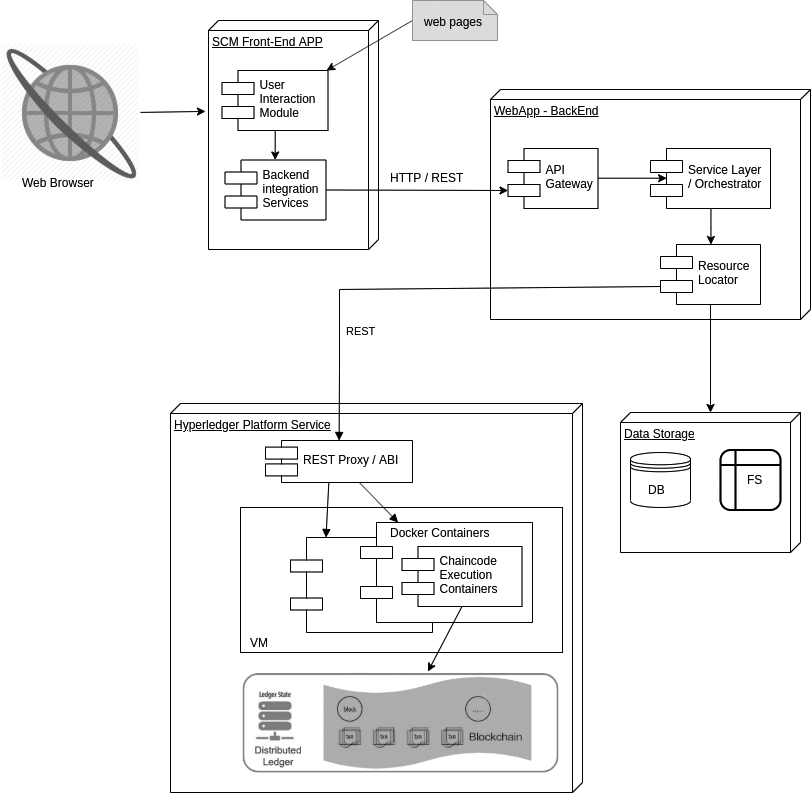
\includegraphics[scale=0.4]{images/detalhamentotecnico.png}
\caption{Árion Application architecture}
\label{fig:detalhamentotecnico}
\end{center}
\end{figure}

\subsection{Frond-End WebApp}\label{sec:WebAppFrondEnd}
Front-End WebApp is a client–server application which the client runs in a web browser. The Front-End Webapp is divided into two main blocks and these are classified according to the interactions: User Interaction Modules and Backend Interaction Services. User Interaction modules are responsible for providing web pages that will be rendered on client’s web browser. The backend interactions happen via a set of services.

\subsection{Back-End WebApp}\label{sec:WebAppBackEnd}
BackEnd - WebApp is a Middleware that runs on the server facilitating the client-server connectivity, forming a middle layer between the app and the network. It contains the logic to send the appropriate data back to the applicant. This module  is composed by the API Gateway, Service Layer and Resource Locator. API Gateway is a managed service that enables easily create, publish, maintain, monitor and secure REST APIs. The service Layer defines its set of available operations from the perspective of interfacing client layers. The service layer acts as an orchestrator, controlling the flow of incoming and outcoming information requests and responses. Resource locators are components that abstracts the persistence layer. Their job is to provide an object that can help services to discover and persist information from/to the Data Storage Module.

\subsection{Data Storage}\label{sec:DataStorage}
Árion uses three applications as data storage: Blockchain, Cloud file system, and relational database. Blockchains grow continuously because of the amount of data and code in them, which is unchanging. Therefore, an important design decision is to choose which data and calculations to keep in and out of the chain. A cloud file system is a tiered storage system that provides shared access to file data. A relational database is a set of formally described tables from which data can be accessed or reassembled in many different ways without having to reorganize the database tables. 

\subsubsection{Blockchain and Chaincode}\label{sec:DataStorageBlockchain}
The platform uses Blockchain to supply chain management tracking parts and service provenance, ensuring authenticity of goods, block counterfeits and reducing conflicts. This usually involves a limited and known number of actors, suggesting use of a permissioned Blockchain, that is, a Blockchain where all nodes must be allowed to be part of the system. To implement that, Hyperledger Fabric is used \cite{cachin2016architecture}. 

Hyperledger Fabric implements smart contracts through chaincode. In general, a smart contract defines the transaction logic that controls the lifecycle of a business object contained in the world state. It is then packaged into a chaincode which is then deployed to a Blockchain network. So, smart contracts rule transactions, whereas chaincode rules how smart contracts are packaged for deployment.

Before businesses transact with each other, they must define a common set of contracts covering common terms, data, rules, concept definitions, and processes. Taken together, these contracts lay out the business model that govern all of the interactions between transacting parties. A smart contract defines the rules between different organizations in executable code. Applications invoke a smart contract to generate transactions that are recorded on the ledger.

